    % specifies the documnt class. We usually use article but there are others. 
\documentclass[a4paper,12pt,oneside]{book}              

% these are standard packages used for the math symbols
\usepackage{amsmath,amssymb,amsthm, enumitem, hyperref, tabto} 
\usepackage[T1]{fontenc}
\usepackage[utf8]{inputenc}
\usepackage[english]{babel}
\usepackage{fancyhdr}
\usepackage{wrapfig}
\usepackage[fleqn]{amsmath}
\usepackage[utf8]{inputenc}
\usepackage{graphicx}
\usepackage{float}
\usepackage[absolute,overlay]{textpos}
\graphicspath{ {./Photos/} }
\usepackage{fancyhdr}
\usepackage[top=1in,bottom=1in,right=1in,left=1in]{geometry}
\usepackage{circuitikz}
\usepackage{tikz}
\usepackage{pgfplots}
\usetikzlibrary{decorations.markings,arrows}
\usetikzlibrary{datavisualization}
\usetikzlibrary{datavisualization.formats.functions}
\pgfplotsset{compat=newest}
\usepackage{amsmath}

% These commands below is to make sure the numbering of these are consistent with theorem
% If you are not sure what something means, delete them, build a new file and see the
% difference between the files. You can ignore this part for now.
\newtheorem{theorem}{Theorem}[section]
\newtheorem{conjecture}[theorem]{Conjecture}
\newtheorem{observation}[theorem]{Observation}
\newtheorem{definition}[theorem]{Definition}
\newtheorem{corollary}[theorem]{Corollary}
\newtheorem{lemma}[theorem]{Lemma}
\newtheorem{example}[theorem]{Example}
\newtheorem{remark}[theorem]{Remark}
\newtheorem{notation}[theorem]{Notation}


% Title of your project
\title{%
  \Huge Calculus \\
  \LARGE  Exploring \textbf{Real} Math
  }

% The author command places text right after title
\author{by \\
\Large The NUS High Math Interest Group (MIG) \\
}

\date{\Large 12th November 2022}

\begin{document}
\maketitle

\tableofcontents

\part{An Introduction}

\newpage
\chapter{Exploring Instantaneous Change}
\vspace{-30pt}
\large \textit{by Jiang Yuzhe}

\subsection{Derivative}
So, What is the definition of a derivative?

\subsection{Notations}
We will be focusing on 2 types of notations that are within out school's syllabus, the Langrange notation and Leibniz notation. 
\subsubsection{Functions (Pre-calculus)}
A function takes in an \textbf{input} and returns an \textbf{output}. However, for any input, the output is \textbf{unique}. For example, if A is the input into the function, and B is an output, then B is the only output of the function. If there are more than 2 outputs for the same input, then it is not a valid function
\subsubsection{Lagrange Notation}
The 1st order derivative of a function is denoted as follows
$$$$


\newpage
\chapter{How do Limits Work?}
\vspace{-30pt}
\large \textit{by Chong How}


\newpage
\chapter{Graphically Understanding the Rules}
\vspace{-30pt}
\large \textit{by Karimi Zayan}

\section{Power rule}

The power Rule states that

$$\frac{d}{dx}(x^n)=nx^{n-1}$$

 \noindent The symbolic proof is as follows
$$
\begin{aligned}
\frac{d}{dx}(x^n)&=\lim_{h\to 0}\frac{(x+h)^n-x^n}{h}\\
&=\lim_{h\to 0}\frac{x^n+\binom{n}{1}x^{n-1}h+\cdots +\binom{n}{n}h^n-x^n}{h}\\
&=\lim_{h\to 0}\frac{\binom{n}{1}x^{n-1}h+\cdots +\binom{n}{n}h^n}{h}\\
&=\lim_{h\to 0}\binom{n}{1}x^{n-1}+\cdots +\binom{n}{n}h^{n-1}\\
&=nx^{n-1}
\end{aligned}
$$

 \noindent To grasp an intuitive sense of this however, we can look at a geometric diagram for the equation $f(x)=x^2$.

\begin{figure}[H]
    \begin{center}
        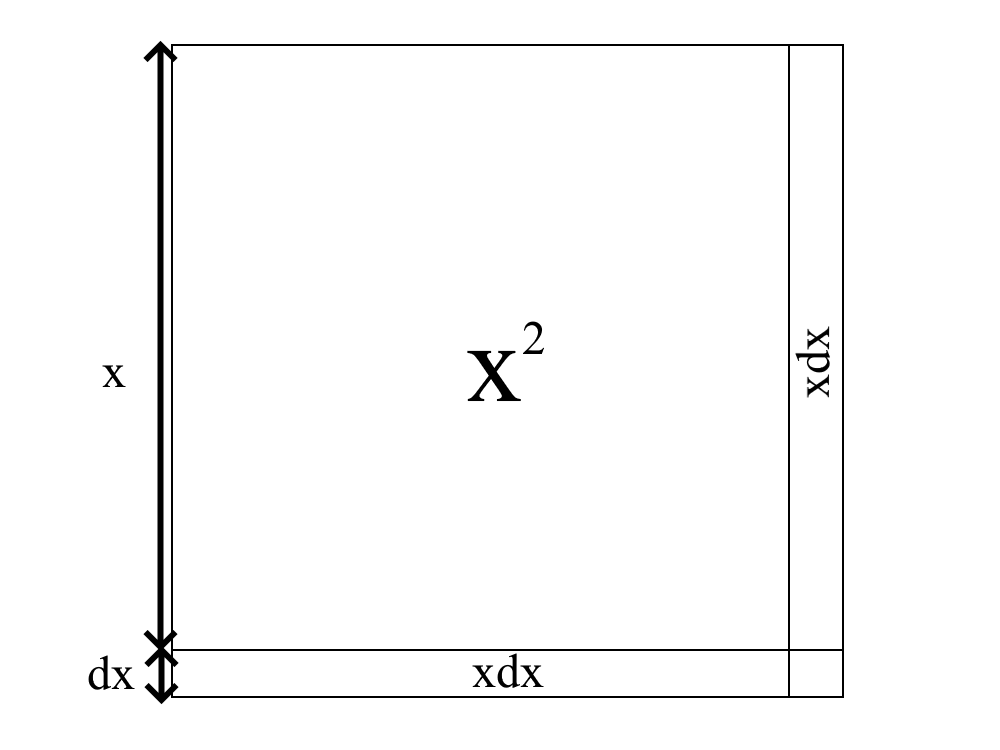
\includegraphics[scale=0.35]{img/zayan/pr1.png}
        \caption{$f=x^2$}
        \label{fig:pr1}
    \end{center}
\end{figure}

 \noindent We look at $x^2$ and if we do a small nudge to $x$ by an infinitesimally small $dx$, we get the diagram as follows. We see that we can obtain an equation for $df$ by summing up the small rectangles that make up the expression.

$$df=xdx+xdx+{dx}^2$$

 \noindent Now, we solve for $\frac{df}{dx}$,
 
$$
\begin{aligned}
df&=xdx+xdx+{dx}^2\\
\frac{df}{dx}&=2x+dx\\
\frac{df}{dx}&=2x
\end{aligned}$$

\noindent We can apply this same logic to a cube.

\begin{figure}[H]
    \begin{center}
        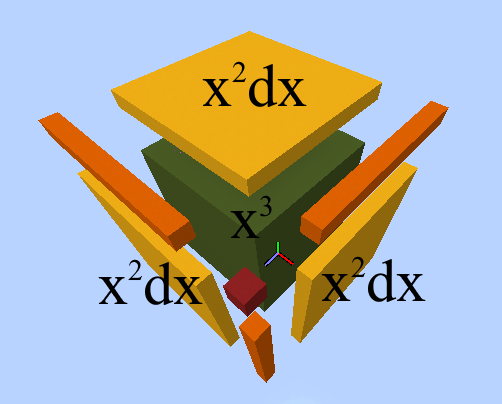
\includegraphics[scale=0.75]{img/zayan/pr2.png}
        \caption{$f=x^3$}
        \label{fig:pr2}
    \end{center}
\end{figure}

\noindent We obtain a new equation for $df$ as follows

$$df = 3x^2dx+3x{dx}^2+{dx}^3$$

\noindent We can easily see

$$\frac{df}{dx}=3x^2$$

\noindent Overall, we see that for any $x^n$, nudging $x$ by $dx$ causes there to be $n$ sections with the value $x^{n-1}dx$ and a varying amount of other sections with areas proportional to $dx^2$ which can be ignored. Hence, we can see easily now why

$$\frac{d}{dx}(x^n)=nx^{n-1}$$

\noindent The power rule defined as such applies for not just integers but also all real numbers. However, the exact proof is beyond the scope of this lesson.

\section{Product rule}

The product rule states that
$$\frac{d}{dx}(f(x)g(x))=f(x)\frac{d}{dx}(g(x))+g(x)\frac{d}{dx}(f(x))$$

\noindent The symbolic proof is as follows

$$
\begin{aligned}
\frac{d}{dx}(f(x)g(x))&=\lim_{h\to 0}\frac{f(x+h)g(x+h)-f(x)g(x)}{h}\\
&=\lim_{h\to 0}\frac{{f({x+h})g({x+h})-f({x+h})g(x)+f({x+h})g(x)-f(x)g(x)}}{h}\\
&=\lim_{h\to 0}f(x+h)\frac{g(x+h)-g(x)}{h}+\lim_{h\to 0}g(x)\frac{f(x+h)-f(x)}{h}\\
&=f(x)\frac{d}{dx}(g(x))+g(x)\frac{d}{dx}(f(x))
\end{aligned}
$$

\noindent To grasp an intuitive sense of this however, we can look at a geometric diagram for the equation $y=f(x)g(x)$ similar to that of $x^2$,

\begin{figure}[H]
    \begin{center}
        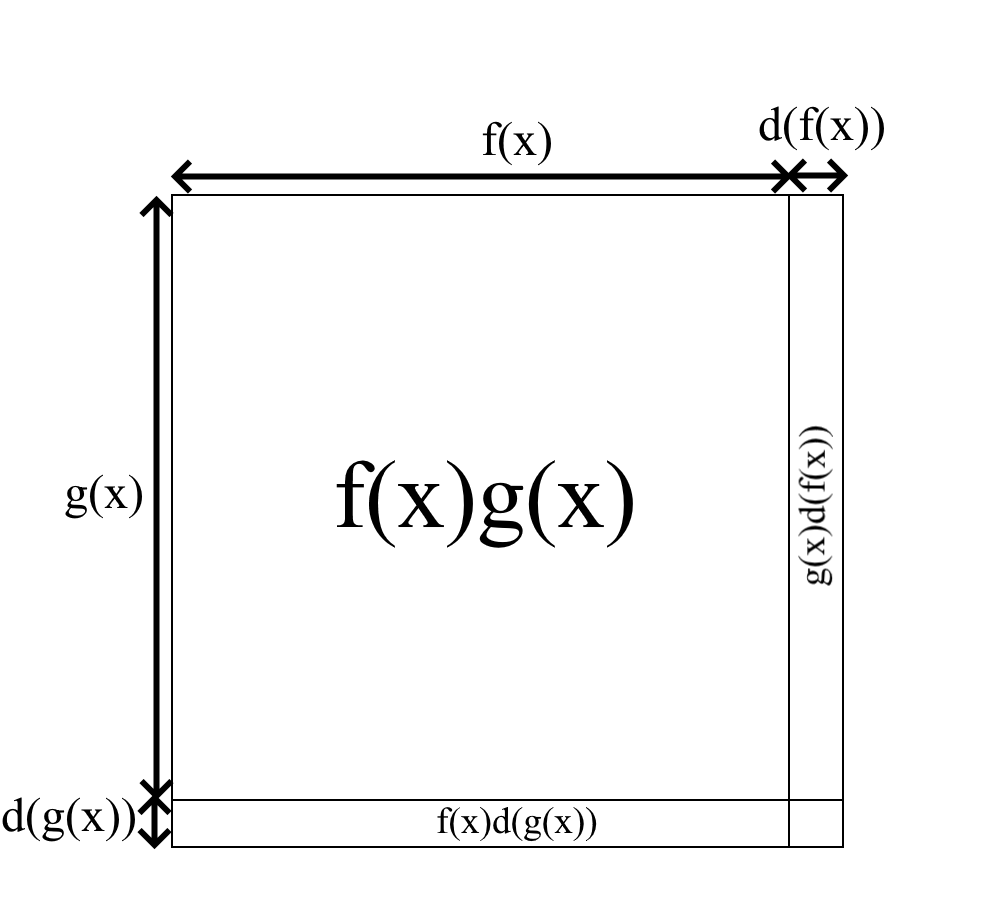
\includegraphics[scale=0.35]{img/zayan/prodrule.png}
        \caption{$y=f(x)g(x)$}
        \label{fig:prodrule}
    \end{center}
\end{figure}

\noindent We set the side lengths to be the functions, hence nudging $x$ by $dx$, the changes in the side lengths will be $d(f(x))$ and $d(g(x))$. We can obtain an expression for $dy$ by summing up all the tiny rectangles

$$dy=f(x)d(g(x))+g(x)d(f(x))+d(g(x))d(f(x))$$

\noindent we now solve for $dy$,

$$\begin{aligned}
dy&=f(x)d(g(x))+g(x)d(f(x))+d(g(x))d(f(x))\\
\frac{dy}{dx}&=f(x)\frac{d}{dx}(g(x))+g(x)\frac{d}{dx}(f(x))+\frac{d}{dx}(f(x))\frac{d}{dx}(g(x))dx\\
\frac{dy}{dx}&=f(x)\frac{d}{dx}(g(x))+g(x)\frac{d}{dx}(f(x))
\end{aligned}$$

\noindent Thus, the product rule is true.

\section{Chain rule}

The chain rule states that

$$\frac{d}{dx}(f(g(x)))=\frac{df(g(x))}{dg(x)}\frac{dg(x)}{dx}$$

\noindent There is no clear geometric proof for this, so I will write one. Define $u$ and $v$ as such

$$u(h)=\left\{ {\begin{array}{*{20}{l}}{\displaystyle \frac{{f( {x + h}) - f( x)}}{h} - \frac{df(x)}{dx}}&{{\mbox{  if }}h \ne 0}\\0&{{\mbox{  if }}h = 0}\end{array}} \right.$$

$$v(h)=\left\{ {\begin{array}{*{20}{l}}{\displaystyle \frac{{g( {x + h}) - g( x)}}{h} - \frac{dg(x)}{dx}}&{{\mbox{  if }}h \ne 0}\\0&{{\mbox{  if }}h = 0}\end{array}} \right.$$

\noindent We see that

$$f(x+h)=f(x)+h\left(u(h)+\frac{df(x)}{dx}\right)$$
$$g(x+h)=g(x)+h\left(v(h)+\frac{dg(x)}{dx}\right)$$

\noindent From this we can extrapolate the rule.

$$\begin{aligned}
\frac{d}{dx}(f(g(x)))&=\lim_{h\to 0}\frac{f(g(x+h))-f(g(x))}{h}\\
&=\lim_{h\to 0}\frac{f(g(x)+h\left(v(h)+\frac{dg(x)}{dx}\right))-f(g(x))}{h}\\
&=\lim_{h\to 0}\frac{f(g(x))+h\left(v(h)+\frac{dg(x)}{dx}\right)\left(u(h\left(v(h)+\frac{dg(x)}{dx}\right))+\frac{df(g(x))}{dg(x)}\right)-f(g(x))}{h}\\
&=\lim_{h\to 0}\frac{h\left(v(h)+\frac{dg(x)}{dx}\right)\left(u(h\left(v(h)+\frac{dg(x)}{dx}\right))+\frac{df(g(x))}{dg(x)}\right)}{h}\\
&=\lim_{h\to 0}\left(v(h)+\frac{dg(x)}{dx}\right)\left(u(h\left(v(h)+\frac{dg(x)}{dx}\right))+\frac{df(g(x))}{dg(x)}\right)\\
&=\frac{df(g(x))}{dg(x)}\frac{dg(x)}{dx}
\end{aligned}$$

\noindent If you don't want to read this a more simpler way to think of it is like this, if a car is moving twice as fast as a bike and a bike is moving 4 times as fast as a person. Then a car is moving 8 times faster than a person. In math form:

$$\frac{dc}{dp}=\frac{dc}{db}\frac{db}{dp}=(2)(4)=8$$

\noindent From the chain rule and product rule, we can basically calculate most derivatives since most functions are products and composites of functions with known derivatives. Hence, by recursively applying these rules, one can solve any problem.

\section{Quotient rule (Optional reading)}

The quotient rule states that

$$\frac{d}{dx}\left(\frac{f(x)}{g(x)}\right) = \frac{g(x)\frac{d}{dx}(f(x))-f(x)\frac{d}{dx}(g(x))}{g^2(x)}$$

\noindent We can prove this by using all the rules we have learnt so far

$$\begin{aligned}
\frac{d}{dx}\left(\frac{f(x)}{g(x)}\right)&=\frac{d}{dx}\left(f(x)\frac{1}{g(x)}\right)\\
&=f(x)\frac{d}{dx}\left(\frac{1}{g(x)}\right)+\frac{\frac{d}{dx}(f(x))}{g(x)}\\
&=-\frac{f(x)}{g^2(x)}\frac{d}{dx}(g(x))+\frac{\frac{d}{dx}(f(x))}{g(x)}\\
&=\frac{g(x)\frac{d}{dx}(f(x))-f(x)\frac{d}{dx}(g(x))}{g^2(x)}
\end{aligned}$$

\part{Physical Applications}

\newpage
\chapter{Movement}
\vspace{-30pt}
\large \textit{by Krishna}


\newpage
\chapter{Displacement}
\vspace{-30pt}
\large \textit{by Favian Lim}


\newpage
\chapter{Area under the Curve}
\vspace{-30pt}
\large \textit{by Ishan Sharma}


\part{Extensions}

\newpage
\chapter{Substituting}
\vspace{-30pt}
\large \textit{by Prannaya Gupta}

Differentiation and Integration often stems from a collective understanding of how small differentials change.

This is known as the 




\end{document}
